\documentclass{article}
\usepackage{graphicx} % Required for inserting images

\title{PS6\_RYU}
\author{Junyeol Ryu}
\date{March 12th 2024}

\usepackage{geometry}

\geometry{
 a4paper,
 left=20mm,
 right=20mm,
 top=20mm,
 bottom=20mm
 }


\begin{document}

\maketitle

\section{Electricity Generation Power Plants using LNG}
\large{This dataset will be utilized for my final project. An associate, currently employed by KEPCO, has graciously provided the dataset for out future research endeavors. The data has already undergone a cleaning process, so it was not necessary to clean it separately.

The dataset encompasses information regarding the characteristics of generators that utilize Liquefied Natural Gas (LNG) for electricity generation, spanning the period from January 2015 to May 2023. It is categorically divided into privately operated companies and nation-operated companies. Private power generation entities directly import LNG from international sources, while nation-operated companies engage in collective importation. Through the analysis of this dataset, we aim to discern the distinct attributes of each importation methodology and ascertain the more cost-effective approach.}
\\


\section{What the images are communicating.
How are they helpful for understanding your dataset?}

\subsection{Figure 1}

\begin{figure}[t]
    \centering
            \caption{Relationship between JKM and JCC}
        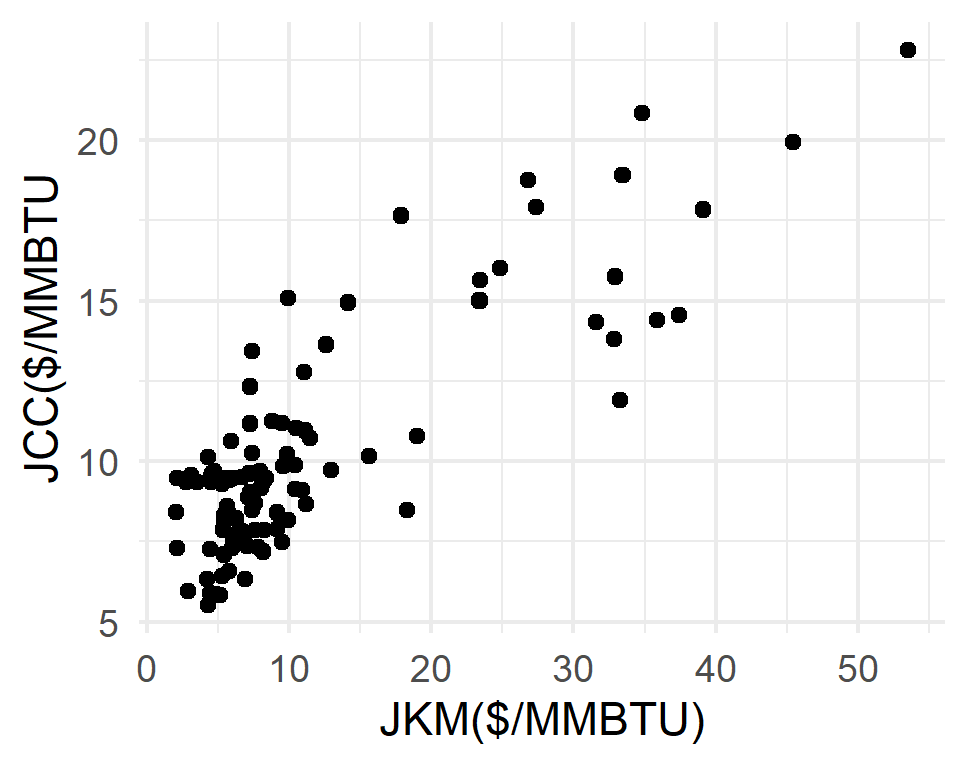
\includegraphics[width=0.5\linewidth]{Figure1.png}
        \label{fig:88mono}
\end{figure}



\large{Figure 1 is a scatterplot showing the relationship between JKM and JCC. The name of JKM is Japan Korea Marker, which is the LNG price index created by S\&P Global Platts in 2009. It is a benchmark price that reflects the spot price of LNG price delivered to Japan, Korea, China, and Taiwan under DES terms. JKM is a price indicator that has a lot of influence on the price of a short-term contract. 
Meanwhile, JCC is Japan Crude Cocktail, which is the Japanese crude oil introduction price based on customs clearance announced by the Japanese Ministry of Commerce. Generally, this indicator has a lot of influence on the price of LNG long-term contracts. 
As we can see, the two energy price indicators show a high positive correlation with each other. For example, if the crude oil price (JCC) rises, the energy cost increases, thus the LNG price (JKM) can also be affected and rise. Conversely, if the crude oil price falls, the LNG price can also fall.}
\\

\subsection{Figure 2}

\begin{figure}[t]
    \centering
            \caption{Relationship between JKM and Fuel Price by Gas Type}
        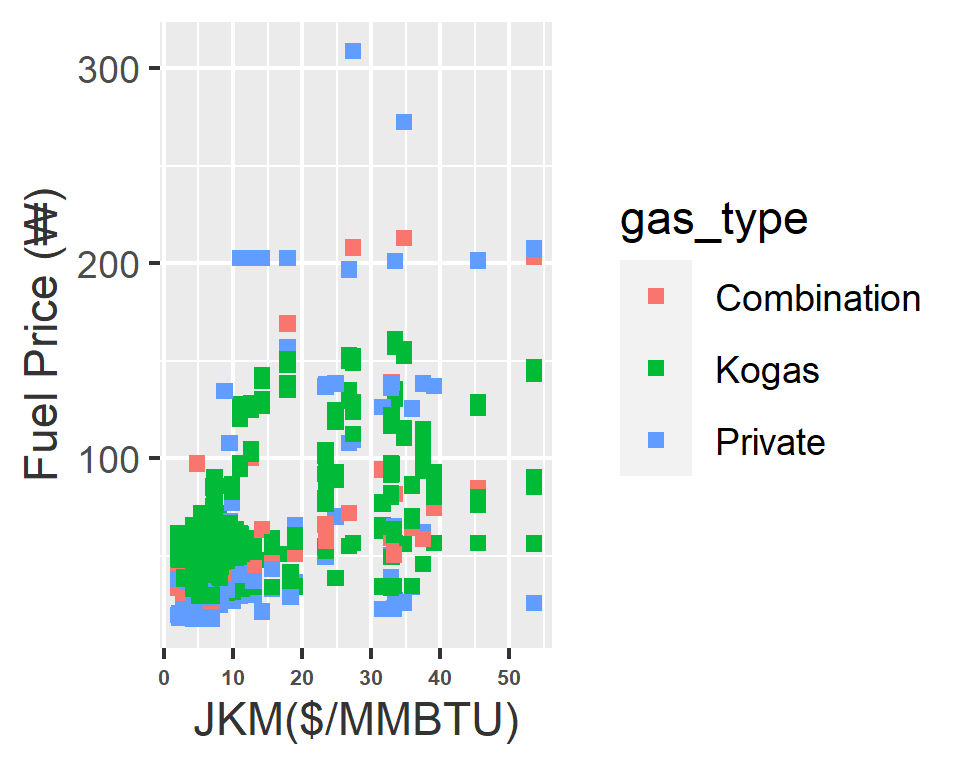
\includegraphics[width=0.5\linewidth]{Figure2.png}
        \label{fig:88mono}
\end{figure}

\large{Figure 2 is showing the data distribution of JKM and the fuel price of each power plant. Fuel Price represents the average cost of electricity generation for each generator using LNG.
"Kogas" represents a generator of a country-run company, "Private" represents a generator operated by a private company, and "Combination" represents a generator using a mixture of the previous two methods. 
As we can see, the distribution of Private is divided into two parts (up and down), and most of the Kogas shows that the variance of fuel price is less than Private. Since private companies purchase LNG individually, each company's bargaining power and purchase timing are different, so such things can be considered to be reflected in high price fluctuations. On the other hand, in the case of the government's joint purchase method, the price deviation was found to be relatively small.}
\\

\subsection{Figure 3}

\begin{figure}[t]
    \centering
            \caption{Fuel Price Histogram by Season}
        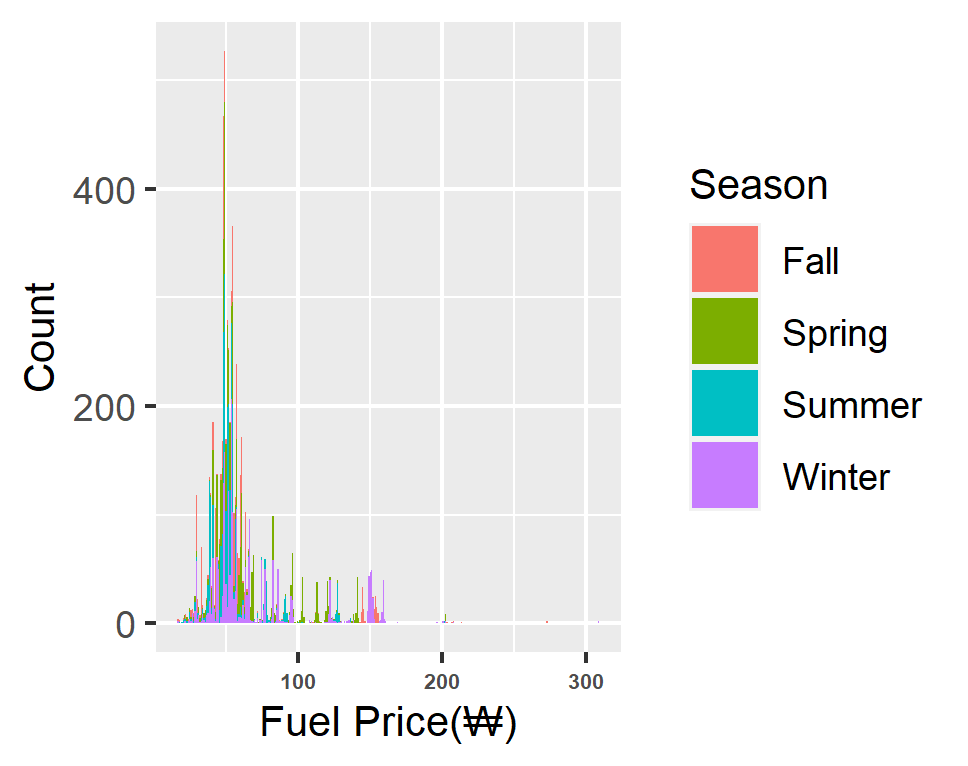
\includegraphics[width=0.5\linewidth]{Figure3.png}
        \label{fig:88mono}
\end{figure}

\large{Figure 3 shows how fuel prices vary from season to season. Since variable costs vary from season to season and fuel prices are affected by variable costs, so fuel prices vary from season to season. 
As we can see, the variation in fuel prices in winter was relatively larger than in other seasons, consistent with our intuition.}
\\


\end{document}
